% Multiple Choice Question 35

\begin{center}
    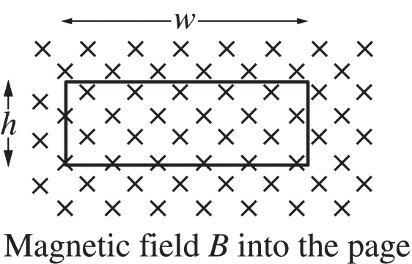
\includegraphics[scale=0.4]{images/img-016-031.png}
\end{center}

\begin{questions}
\setcounter{question}{34}

\question
A wire loop with width $w$ and height $h$ is in a magnetic field that is directed into the page, as shown in the figure above. The magnitude $B$ of the magnetic field changes with time $t$. The magnitude of the resulting induced emf in the wire loop is given as a function of time by the equation $\varepsilon=\beta h w t^{3}$, where $\beta$ is a positive constant in units of $\mathrm{T} / \mathrm{s}^{4}$. Which of the following is a possible expression for the magnitude of the magnetic field?

\begin{oneparchoices}
    \choice $\dfrac{1}{4} \beta t^{3}$
    \choice $3 \beta t^{4}$
    \choice $3 h w \beta t^{2}$
    \choice $\dfrac{1}{4} h w \beta t^{4}$
    \choice $\dfrac{1}{4} \beta t^{4}$
\end{oneparchoices}

\end{questions}
